\chapter{Testing and Experimenting}


\section{Overall approach to testing and experiments}
In the sense of this project testing was carried out for multiple purposes. From a software development point of view testing was carried out to ensure that the app performed as expected, whereas from the research perspective of this project, testing was carried out to determine whether hybrid apps are feasible alternatives to native apps.

The acceptance and unit testing was carried out to test the functionality of the app and that the software performs as expected. The user testing and resource testing was more the experimental side as it helped answer the research element to this project.

\section{Acceptance Testing}
It was important that all of the stories and features of the app worked properly as this would help with user testing. Whilst there was no business or end user, to specify project requirements, these were devised from the initial stories. Table 4.1 was derived which broke down all of the stories into multiple different features. These features were then tested, and a comment was left if the test did not pass.

\begin{center} 
 \begin{tabular}{||c c c c||}  
 \hline
 Story & Feature Name & Pass/Fail & Comment \\
 \hline\hline
 Registration and Login & Register user details &  Fail &  \begin{tabular}{@{}c@{}} User's postcode \\ does not get\\ added properly \end{tabular} \\
 \hline
 Registration and Login & \begin{tabular}{@{}c@{}}Login with \\ previously created \\ account \end{tabular} & Pass &  Works as expected \\
 \hline
 Registration and Login & Logout & Fail & \begin{tabular}{@{}c@{}} System appears to \\ logout okay however \\ it loads the previous \\ user's feed \end{tabular} \\
 \hline
 Profile Page & \begin{tabular}{@{}c@{}} Upload picture \\ from library \end{tabular}  &  Pass  & Works as expected  \\ 
 \hline
Profile Page & \begin{tabular}{@{}c@{}}Take picture \\using device's camera \\ and upload.\end{tabular} & Pass &  Works as expected  \\ 
\hline
Profile Page & Update bio & Pass & Works as expected \\
\hline 
Post System & User Posts & Pass &  \begin{tabular}{@{}c@{}} User posts get \\ added to feed table \\ as expected \end{tabular} \\
\hline
Follow System & \begin{tabular}{@{}c@{}} User can follow \\ other users \end{tabular} & Pass &  \begin{tabular}{@{}c@{}} Adds data to \\ the correct table \\ and shows as followed \\ on the app \end{tabular} \\
\hline
Follow system &  \begin{tabular}{@{}c@{}} User can unfollow \\ other users \end{tabular} & Pass &  \begin{tabular}{@{}c@{}} Can successfully unfollow other users \end{tabular} \\
\hline
 \begin{tabular}{@{}c@{}} Post System \\ and Follow System \end{tabular} &  \begin{tabular}{@{}c@{}} Correct posts \\ display on user's \\ home page \end{tabular} & Pass & The correct posts display \\
 \hline
 Create Events System & Create a Venue & Pass &  \begin{tabular}{@{}c@{}} All necessary details \\ are stored in the \\ back end appropriately \end{tabular} \\
\hline
 Create Events System & Create Events  & Pass & \begin{tabular}{@{}c@{}} Events are \\ properly created \\ and have a correct \\ link to the appropriate \\ venue id \end{tabular} \\
 \hline
 Search &  \begin{tabular}{@{}c@{}} User can search \\ for nearby events \end{tabular} & Pass &  \begin{tabular}{@{}c@{}} Uses device's GPS \\ correctly and compares \\ with event's location \end{tabular} \\
 \hline
  Search &  \begin{tabular}{@{}c@{}} User can search \\ for nearby music \\ lovers and artists \end{tabular} & Pass &  \begin{tabular}{@{}c@{}} Uses device's GPS \\ correctly and compares \\ with user's location \end{tabular} \\
  \hline
  \hline
 \end{tabular}
   \end{center}
  \begin{center} 
 \begin{tabular}{||c c c c||}  
 \hline
 Story & Feature Name & Pass/Fail & Comment \\
 \hline\hline

   Search &  \begin{tabular}{@{}c@{}} User can search \\ for events \\ which are happening \\ soon \end{tabular} & Pass &  \begin{tabular}{@{}c@{}} Correctly sorts \\ events by dates  \end{tabular} \\
  \hline
  \hline
\end{tabular}
\end{center}
 \captionof{table}{User Acceptance Testing Table}
\vspace{5mm}

It is clear from Table 4.1 that in terms of acceptance testing some of the code contained bugs, for example the logout system was not working properly. Once all of the issues in Table 4.1 had been addressed, another table, Table 4.2 was created. This repeats the tests which failed in Table 4.2 and evaluates whether they now pass.

\begin{center} 
 \begin{tabular}{||c c c c||}  
 \hline
 Story & Feature Name & Action Taken & Now Pass/Fail \\
 \hline\hline
 Registration and Login & Register User Details & \begin{tabular}{@{}c@{}} API amended \\ so that the \\ postcode variable \\ is now assigned \\ properly \end{tabular} & Pass \\
 \hline
 Registration and Login & Logout & \begin{tabular}{@{}c@{}} Now clears \\ cache on logout \end{tabular} & Pass \\
 \hline
 \end{tabular}
 \end{center}
 \captionof{table}{Corrections of failures from initial user acceptance testing}

\section{Unit tests}
It is important to unit test each of the main functions within the controllers to make sure that the user of the app will not encounter any unintended behaviour. The Jasmine and Karma frameworks were used for unit testing the app \cite{testing}.

Figure 4.1 gives a small extract of the login unit test which was written (the whole logintest.js file can be found in the appendix). This unit test tests the login controller. The unit tests work in such a way that the developer describes the function, followed by saying what the function should do and finally what happens if the function goes wrong. 

\begin{figure}[H]

\begin{verbatim}
describe('#doLogin', function() {
  it('Should Login using correct details', function() {
    expect(loginMock.doLogin).toHaveBeenCalledWith
    ('sea6@aber.ac.uk', 'b261la'); 
  });

  describe('when the login action is performed,', function() {
    it('if successful, should change state to home', function() {
      expect(stateMock.go).toHaveBeenCalledWith('app.home');
    });

    it('if unsuccessful, should show a popup', function() {
      expect(ionicPopupMock.alert).toHaveBeenCalled();
    });
  });
})
\end{verbatim}
\caption{Sample of unit test for login}
\end{figure}

Table 4.3 illustrates the different unit tests which were created and what functions were tested using these unit tests. Not every function was tested as some functions were very similar to functions in other controllers.

\begin{tabular} {||c c c c||}  
\hline
 Controller Name & Function Tested & What should happen & Name of Testing File\\
 \hline
 \hline 
 Login & doLogin & Login with details & logintest.js \\
 \hline
 Login & register &Move to registration screen & logintest.js \\
 \hline
 Register & doRegistration & Register with details & registertest.js \\
 \hline
 Register & returnToLogin & Change state to login & registertest.js \\
 \hline
 Home & postStatus & Post a status and popup should appear & hometest.js \\
 \hline
 \end{tabular}
  \captionof{table}{Table which shows different unit tests}


\section{User Interface testing}
For a mobile app, user interface testing is very important. As the user interface is essentially how the user navigates around the front end and how they submit data to the back end. Whilst there is no simple automatic way to test the UI on an ionic application, a table as shown in Figure 4.4 was derived which shows all of the different buttons and navigation options to ensure that the UI worked as expected.

\begin{center} 
 \begin{tabular}{||c c c c||}  
 \hline
 Location & Button/Navigation & Pass/Fail & Comment \\
 \hline
 Login Screen & Register Button & Pass & \begin{tabular}{@{}c@{}} Takes user to registration \\ screen as expected \end{tabular} \\
 \hline
 Login Screen & Login Button & Pass & \begin{tabular}{@{}c@{}} Logs the user \\ in if credentials are \\ correct, if not it \\ displays an error message \end{tabular} \\
 \hline
 Registration Screen & Return to Login Button & Pass & \begin{tabular}{@{}c@{}} App returns to \\ login screen on button \\ click \end{tabular} \\
 \hline
 Registration Screen & Register Button & Pass & \begin{tabular}{@{}c@{}} Creates an account \\ if user has entered \\ correct information or \\ displays an error if \\ invalid information entered \end{tabular} \\
 \hline
 \begin{tabular}{@{}c@{}} Menu (Shared across \\ multiple pages once \\ user is logged \\ in) \end{tabular} & Home link & Pass & \begin{tabular}{@{}c@{}} Take user to \\ the home page \end{tabular} \\
 \hline
 \begin{tabular}{@{}c@{}} Menu (Shared across \\ multiple pages once \\ user is logged \\ in) \end{tabular} & Artists link & Pass & \begin{tabular}{@{}c@{}} Takes user to \\ artists page \end{tabular} \\
 \hline
 \begin{tabular}{@{}c@{}} Menu (Shared across \\ multiple pages once \\ user is logged \\ in) \end{tabular} & Events link & Pass & \begin{tabular}{@{}c@{}} Takes user to \\ events page \end{tabular} \\
 \hline
 \begin{tabular}{@{}c@{}} Menu (Shared across \\ multiple pages once \\ user is logged \\ in) \end{tabular} & Music Lovers link & Pass & \begin{tabular}{@{}c@{}} Takes user to \\ music lovers page \end{tabular} \\
 \hline
 \begin{tabular}{@{}c@{}} Menu (Shared across \\ multiple pages once \\ user is logged \\ in) \end{tabular} & My Profile link & Pass & \begin{tabular}{@{}c@{}} Takes user to \\ my profile page. \end{tabular} \\
 \hline
 \begin{tabular}{@{}c@{}} Menu (Shared across \\ multiple pages once \\ user is logged \\ in) \end{tabular} & Logout link & Pass & \begin{tabular}{@{}c@{}} Logs user out \\ and returns them \\ to login page \end{tabular} \\
 \hline
 \begin{tabular}{@{}c@{}} Menu (extras only \\ for venue owners) \end{tabular}& Add a venue link & Pass & \begin{tabular}{@{}c@{}} Takes venue owner \\ to add a \\ venue page \end{tabular} \\
 \hline
 \begin{tabular}{@{}c@{}} Menu (extras only \\ for venue owners) \end{tabular}& Make event link & Pass & \begin{tabular}{@{}c@{}} Takes venue owner \\ to add an \\ event page \end{tabular} \\
 \hline
Home Page & Submit post button & Pass & \begin{tabular}{@{}c@{}} Button posts the \\ data as expected\end{tabular} \\
 \hline
 \hline
  \end{tabular}
   \end{center}
     \begin{center} 
 \begin{tabular}{||c c c c||} 
    \hline
 Location & Button/Navigation & Pass/Fail & Comment \\
 \hline
 Artists & \begin{tabular}{@{}c@{}} Sort by Recommended \\ Music Lovers \end{tabular} & Pass & Displays correct results \\
 \hline

Artists & \begin{tabular}{@{}c@{}} Sort by Nearby \\ Music Lovers \end{tabular} & Pass & Displays correct results \\
 \hline
Artists & \begin{tabular}{@{}c@{}} Sort by Newly \\ Joined Music Lovers \end{tabular} & Pass & Displays correct results \\
\hline
Artists & \begin{tabular}{@{}c@{}} Click more info\\ link on a \\ artist \end{tabular} & Pass & \begin{tabular}{@{}c@{}} Correctly navigates to \\ the individual artist's \\ page \end{tabular} \\
 \hline
Artist Individual Page & \begin{tabular}{@{}c@{}} Follow button \end{tabular} & Pass & Correctly follows artist. \\
 \hline
Artist Individual Page & \begin{tabular}{@{}c@{}} Un Follow button \end{tabular} & Pass & Correctly unfollows artist. \\
  \hline
Events & \begin{tabular}{@{}c@{}} Sort by \\ Recommended Events \\ selected and sort \\ button clicked\end{tabular} & Pass & Correctly sorts the events \\
 \hline
 Events & \begin{tabular}{@{}c@{}} Sort by \\ Nearby Events \\ selected and sort \\ button clicked\end{tabular} & Pass & Correctly sorts the events \\
 \hline
 Events & \begin{tabular}{@{}c@{}} Sort by \\ Near Your Home \\ selected and sort \\ button clicked\end{tabular} & Pass & Correctly sorts the events \\
 \hline
 Events & \begin{tabular}{@{}c@{}} Sort by \\ Date of Events \\ selected and sort \\ button clicked\end{tabular} & Pass & Correctly sorts the events \\
 \hline 
 Events & \begin{tabular}{@{}c@{}}More info pressed \\ on event \end{tabular} & Pass & \begin{tabular}{@{}c@{}} Correctly navigates \\ to the individual \\ event \end{tabular} \\
 \hline
 Individual Event & \begin{tabular}{@{}c@{}}Add event to favourites \\ clicked on event. \end{tabular} & Pass & \begin{tabular}{@{}c@{}} Correctly adds event \\ to user favourites \end{tabular} \\
 \hline 
Individual Event & \begin{tabular}{@{}c@{}}Remove event from favourites \\ clicked on event \end{tabular} & Pass & \begin{tabular}{@{}c@{}} Correctly removes event \\ from favourites \end{tabular} \\
 \hline
Add a venue & Register venue button pressed & Pass & \begin{tabular}{@{}c@{}} Creates venue on \\ button click or displays \\ error message if fields \\ are missing \end{tabular} \\
\hline
Add an Event & Register event button pressed  & Pass & \begin{tabular}{@{}c@{}} Creates event on \\ button click or displays \\ error message if fields \\ are missing \end{tabular} \\
\hline
\hline
 \end{tabular}
  \end{center}
 \begin{center}
 \begin{tabular}{||c c c c||}  
    \hline
     Location & Button/Navigation & Pass/Fail & Comment \\
     \hline \hline
General & User swipes screen left  & Pass & \begin{tabular}{@{}c@{}} Shows menu \\ as expected \end{tabular} \\
\hline
General & \begin{tabular}{@{}c@{}} User swipes screen right \\ when menu open \end{tabular} & Pass & \begin{tabular}{@{}c@{}} Closes menu \\ as expected \end{tabular} \\
\hline
\hline
 \end{tabular}
 \end{center}
  \captionof{table}{UI testing table}

\section{User testing}
In terms of user testing, the questions which were discussed in the experimental methods section (see Appendix 4), were measured on a scale of 1 to 10, with 10 meaning that the user found the hybrid app fast and 1 meaning it was slow. Table 4.5 shows the results.

\begin{center} 
 \begin{tabular}{||c c c c c c c||}  
 \hline
  \hline
 Participant & Q1 & Q2 & Q3 & Q4 & Q5 & Q6 \\
 \hline
 1 & 8 & 7 & 9 & 6 & 8 & 6 \\
 \hline
 2 & 9 & 6 & 8 & 4 & 9 & 9 \\
 \hline
 3 & 10 & 9 & 9 & 4 & 8 & 4 \\
 \hline
 4 & 8 & 4 & 5 & 2 & 6 & 3 \\
 \hline
 5 & 9 & 5 & 6 & 4 & 9 & 7 \\
 \hline
 6 & 8 & 6 & 8 & 5 & 8 & 7 \\
 \hline
 7 & 6 & 5 & 3 & 2 & 7 & 5 \\ 
 \hline
 8 & 9 & 6 & 4 & 4 & 8 & 6 \\
\hline
\hline
 \end{tabular}
 \end{center}
\captionof{table}{User Tests Table}

 \subsection{Statistical breakdown of questions}
 Each of these questions was broken down and statistically analysed; the mean, range and standard deviation was established. This helped understand not only how different people have different opinions about the speed and usability of the hybrid app technology but also aided in determining what the overall feeling about each question is.
 \begin{enumerate}
  \item Question 1 - The mean for this question was 8.375, the range was 3 and the standard deviation was 1.18773.
  \item Question 2 - The mean for this question was 6, the range was 4 and the standard deviation was 1.51186.
  \item Question 3 - The mean for this question was 6.5, the range was 6 and the standard deviation was 2.32993.
  \item Question 4 - The mean for this question was 3.875, the range was 4 and the standard deviation was 1.3562.
  \item Question 5 - The mean for this question was 7.875, the range was 3 and the standard deviation was 0.99103.
  \item Question 6 - The mean for this question was 5.875, the range was 5 and the standard deviation was 1.88509.
\end{enumerate}

Figure X (created using \url{http://www.alcula.com/calculators/statistics/box-plot/}) gives each of the questions answers broke down into a box plots.
\begin{center}
\begin{figure}[H]
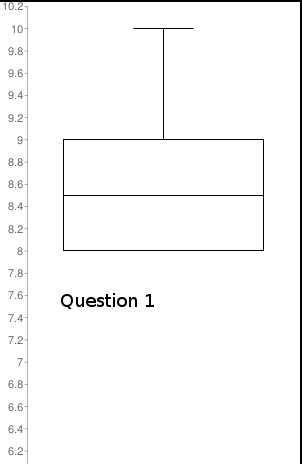
\includegraphics[scale=0.45]{images/q1}
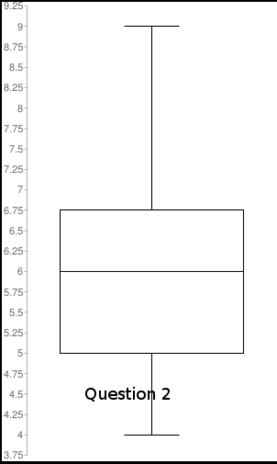
\includegraphics[scale=0.45]{images/q2}
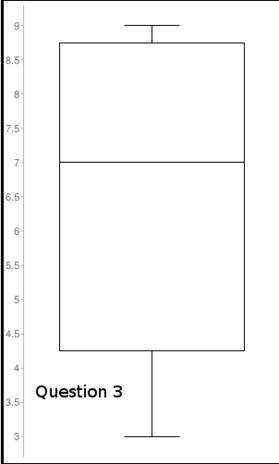
\includegraphics[scale=0.45]{images/q3}
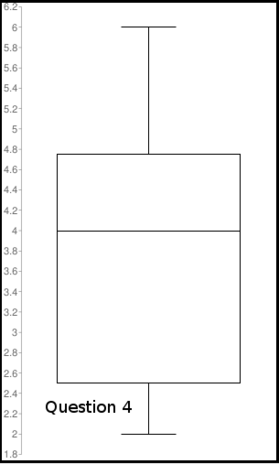
\includegraphics[scale=0.45]{images/q4}
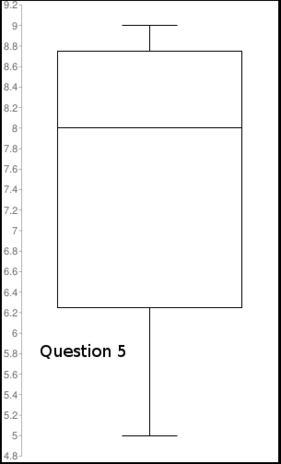
\includegraphics[scale=0.45]{images/q5}
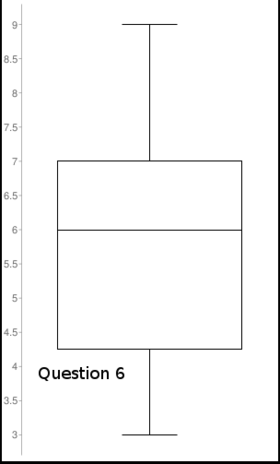
\includegraphics[scale=0.45]{images/q6}
\caption{Box plots which give a visual representation of answers}
\end{figure}
\end{center}
From this data it is clear that different people have varying opinions on the performance of the hybrid app which was developed. The answers to the questions as a whole generally gave a positive response. It is apparent from the questions that users of the app do feel that the camera functionality is slower than a native app.

 \section{Resource usage}
 When considering the hybrid mobile application it is also important to consider how much of the device's resources the app is using. For comparison the resource usage of Facebook has also been listed (this is because Facebook is a native app).

 One of the resources which was compared was the amount of CPU, (as shown in Figure 4.3) when Facebook was looking for events it used 6\% whereas when the hybrid app also used 6\% when looking for events. It does need to be considered that Facebook is significantly larger than the hybrid app which was created consequently the hybrid app uses more CPU for less data than Facebook. Figure 4.3 illustrates this.

\begin{figure}[H]
\begin{center}
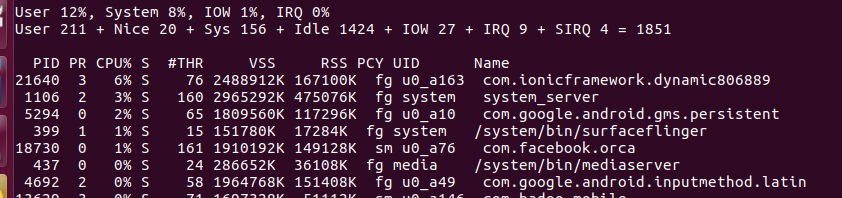
\includegraphics[scale=0.45]{images/ram2}
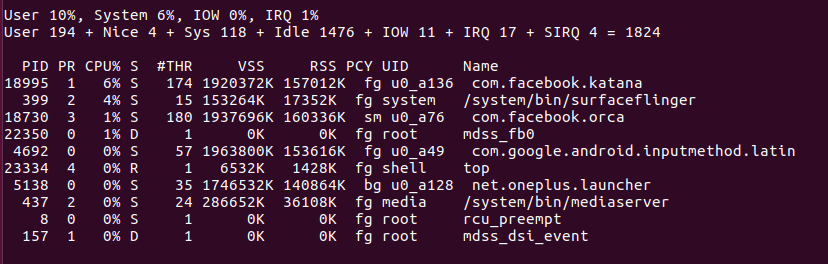
\includegraphics[scale=0.45]{images/ram3}
\caption{Images showing Facebook and Dynamic CPU.}
\end{center}
\end{figure}

The actual amount of storage the app uses is rather high when considering the app stores very little local data. This is mainly due to how ionic does caching. The app, after being installed and a user going through different elements of the app, uses 13.73MB (as shown in Figure 4.4) of a device's storage which is rather large considering most things are stored on the back end rather than on the phone itself. 

\begin{center}
\begin{figure}[H]
\begin{center}
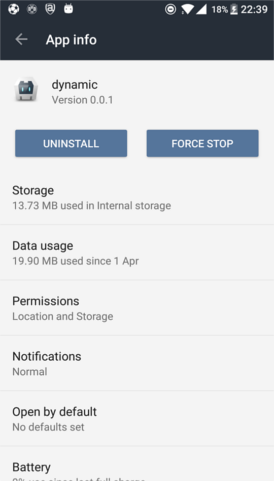
\includegraphics[scale=0.5]{images/usage}
\caption{Resource Usage}
\end{center}
\end{figure}
\end{center}

The amount of storage the app is using is a clear disadvantage to developing apps in a hybrid manner as developing apps in a native manner would give the developer more control over the amount of resources being used.

\section{Conclusion of testing}
The software development side of this project was a success as both the user acceptance testing and the unit tests passed. The user testing for determining whether hybrid apps are feasible alternatives to native apps was positive. From the multiple answers to the various questions asked it seems clear that users of the app are satisfied with it. Therefore, it would be reasonable to conclude that developing a mobile application in a hybrid manner is a feasible alternative to developing mobile applications in a native manner. When a comparison to Facebook has been made it does need to be considered that Facebook is a substantially larger system and has a lot more data. 

